\subsection{The four episodes and their shocks}\label{sec:episodes}

Three shocks are taken from published sources, with their citations
and attribution caveats, and not re-estimated; the tariff shock is an
assumed scenario. The four differ on every dimension the comparison
uses: two are adverse price shocks, one an adverse earnings shock and
one a price gain; two are estimated or observed, one is projected and one is assumed;
one is transmitted through the terms of trade and three are policy
acts. Figure~\ref{fig:episode-map} places them by channel and sign, and
Table~\ref{tab:first-stages} lists each with its source and status.

\begin{figure}[!htb]\centering
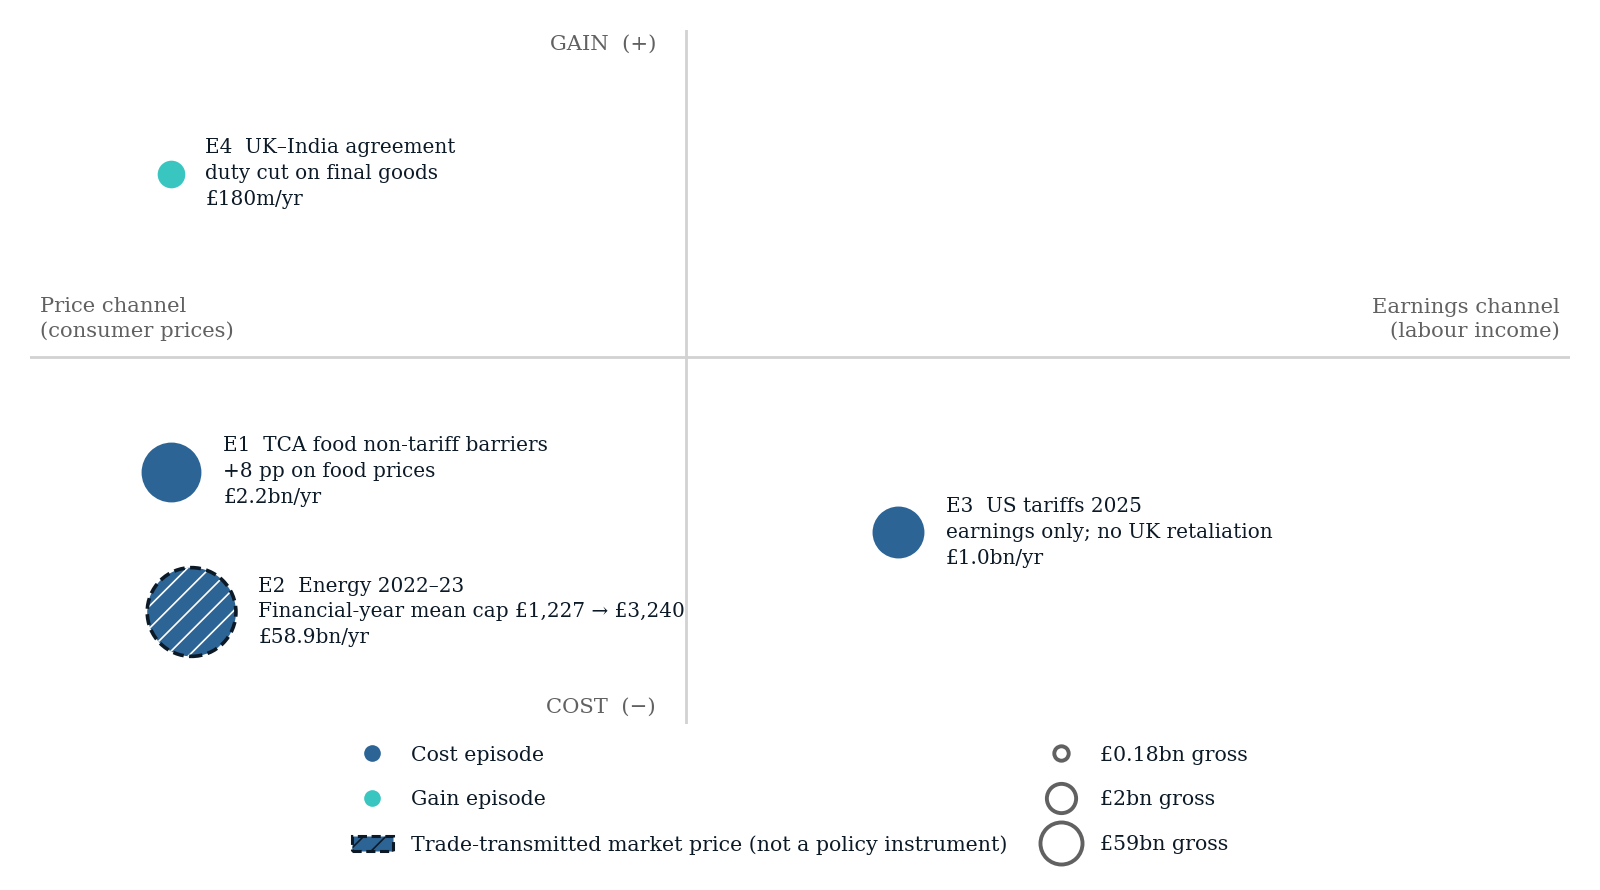
\includegraphics[width=0.9\textwidth]{figures/fig_episode_map.png}
\caption{The four episodes by channel and sign. Bubble area is log-scaled in shock size (energy: the counterfactual shock). Positions are classifications, not measurements.}
\label{fig:episode-map}
\end{figure}

\subsubsection{Episode 1: the TCA border (2021--23)}

The TCA took effect in January 2021,
replacing single-market membership with a border that is tariff-free
but carries non-tariff barriers. The price evidence is
quasi-experimental: exploiting cross-product variation in EU import
intensity, \citet{bakker2023} attribute roughly 8 percentage points of
the 25 per cent food-price rise between December 2019 and March 2023
to those barriers, a cumulative \pounds 250 per household on food
alone, \pounds 6.95 billion in aggregate (their household count;
\pounds 250 on the ONS count used here gives \pounds 7.1 billion),
with pass-through of barrier costs to consumers of 50--80 per cent and
the largest effects in high-EU-import products such as meat and dairy.
Their estimation window opens in December 2019, thirteen months before
the TCA took effect; the episode is dated 2021--23 here and the
pre-entry months enter as zeros. The March 2026 revision of the same
study, an unpublished working paper, raises the estimate to a 4 per
cent rise a year and 12 per cent over three years, with household
losses of \pounds 14.8 billion \citep[\pounds 536 per household;][]{bakker2026}. The paper stays on the 2023 estimate, whose
\pounds 250 cumulative anchors the headline path, so the level of the
food episode should be read as the lower of the two.

The identification is relative, across products, so economy-wide
effects may be missed. On the trade side, UK imports from the EU fell
about 25 per cent in relative terms on entry \citep{freeman2022}, and
in 2022 goods exports were an estimated \pounds 27 billion (6.4 per
cent) below counterfactual, with some 16,400 firms exiting EU
exporting entirely \citep{freeman2024}. The earnings side, by
contrast, rests on assumptions rather than estimates (the standing assumptions of the Office for Budget Responsibility
(OBR), a 15 per cent fall in trade intensity and a 4 per cent fall in
productivity; \citealp{obrbrexit}) and is not carried here.

% Generated by figures/make_figures.py -- do not edit by hand.
% Requires: \usepackage{booktabs}  (no other package needed)
% \rr = ragged-right inside a p{} cell, with \\ restored as the row
% terminator, so narrow columns neither overfull nor stretch-underfull.
\providecommand{\rr}{\raggedright\let\\\tabularnewline}

\begin{table}[tbp]
\centering
\footnotesize
\setlength{\tabcolsep}{3pt}
\renewcommand{\arraystretch}{1.15}
\caption{The four shocks: source and status}
\label{tab:first-stages}
\begin{tabular}{@{}p{1.75cm} p{1.70cm} p{1.45cm} p{2.30cm} p{2.10cm} p{2.75cm} p{1.85cm}@{}}
\toprule
\rr Episode & \rr Date & \rr Type & \rr Channel & \rr Source & \rr Key number & \rr Status \\
\midrule
\rr E1 TCA food non-tariff barriers & \rr Dec 2019--\newline Mar 2023$^{w}$ & \rr Policy & \rr Consumer prices (food) & \rr \citet{bakker2023} & \rr $+8$ pp on food prices & \rr Estimate\newline (ex post) \\[3pt]
\rr E2 Energy 2022--23 & \rr Apr 2022--\newline Mar 2023 & \rr Market & \rr Consumer prices (energy) & \rr \citet{ofgem2021, ofgem2022, ofgemcap2023}; \citet{obrenergy2023} & \rr FY-mean cap \pounds\SsBaseFyCap\ $\to$ \pounds\SsCounterFyCap\ (\pounds\SsRealisedFyCap\ with the Guarantee) & \rr Observed\newline (statutory) \\[3pt]
\rr E3 US tariffs 2025 & \rr 2025--26 & \rr Policy\newline (foreign) & \rr Earnings only; no UK retaliation & \rr Constructed here (Appendix~\ref{app:e3}) & \rr \pounds\MsUSTariffGrossShockMillions m/yr earnings loss (unit elasticity) & \rr Scenario\newline (assumed) \\[3pt]
\rr E4 UK--India agreement & \rr 2026-- & \rr Policy & \rr Consumer prices (clothing, footwear, food) & \rr \citet{dbtindia2026} & \rr \pounds180m/yr duty cut on final goods & \rr Projection\newline (ex ante) \\[3pt]
\bottomrule
\end{tabular}

\vspace{2pt}
\begin{minipage}{\linewidth}\footnotesize
\emph{Notes.} Type distinguishes a policy instrument from a
market price imported through the terms of trade. E3's consumer-price effect is exactly zero (the UK imposed no
retaliatory tariffs), so its household incidence runs through earnings alone.
$^{w}$~the \emph{estimation} window of the cited study; the TCA itself
entered into force in January 2021.
\end{minipage}
\end{table}


\subsubsection{Episode 2: the terms-of-trade shock (2022--23)}

The 2022 energy and import-price surge was, in the Bank of England's
description, a terms-of-trade shock of a size unseen since the
mid-1970s: the terms of trade deteriorated 6.2 per cent in the year to
2022Q3 \citep{onstot2023}, and import prices rose 20 per cent relative
to output prices over two years \citep{broadbent2022}. The energy
import bill roughly doubled to \pounds 117 billion in 2022
\citep{oeuk2023}, the increase of roughly \pounds 60 billion being a
transfer abroad of about 2.5 per cent of GDP (author's calculation),
and of the roughly 17 per cent CPI rise to 2022Q4 more than 70 per
cent (12.7 points) was imported \citep{dhingrapage2023}.

The household price vector is observed and policy-mediated. Ofgem's
cap on a typical annual bill rose from \pounds 1,277 (winter 2021--22)
to \pounds 1,971 (April 2022), \pounds 3,549 (October 2022) and
\pounds 4,279 (January 2023) \citep{ofgem2021, ofgem2022, ofgemcap2023}, and the
Energy Price Guarantee held it at \pounds 2,500 from
October 2022, at an ex-ante cost the OBR put at \pounds 27 billion
within \pounds 47 billion of price subsidies and \pounds 78 billion of
total energy support \citep{obrenergy2023}. \citet{levell2025} put
counterfactual no-policy welfare losses at 6 per cent of income on
average, with some households facing much larger losses. This is the
best-measured shock of the four, with independent official figures for
both the aggregate shock and the retail price vector and a published
decomposition of the cap. The paper therefore measures the shock
before policy and treats the Guarantee and the other legislated
instruments as responses to it, so that automatic and discretionary
cushioning can be separated.

\subsubsection{Episode 3: the US tariffs (2025--26)}

The April 2025 US schedule, before any mitigation, set a 10 per cent
baseline and 25 per cent on motor vehicles and steel
\citep{boempr2025}. Because
pass-through of US tariffs to US import prices is close to complete
\citep{amitireddingweinstein2019, fajgelbaumetal2020, cavalloetal2021},
the UK effect runs through export demand and earnings rather than UK
consumer prices; the UK had imposed no retaliatory tariffs as of
November 2026, so the consumer-price side of this episode is zero. The
earnings scenario is constructed here
(Section~\ref{sec:results-tariff}; Appendix~\ref{app:e3}), on the same
microdata and model version as the price episodes. Each Standard Industrial Classification (SIC) division's
employee wage bill falls by the tariff rate times the US-export share
of turnover times an export-demand elasticity times the wage-bill
incidence, with the elasticity and the incidence both set to one as a
benchmark, not an estimate. The resulting earnings loss is
\pounds\MsUSTariffGrossShockMillions\ million a year.

The external reference points are the OBR's March 2025 scenarios
\citep[import-demand elasticity 0.4; peak GDP effects of $-0.6$ to
$-1.0$ per cent;][]{obr2025} and the Bank of England's estimate of an
effective US tariff on UK goods of about 11 per cent at April 2025
\citep{boempr2025}. At the OBR's elasticity the loss falls to about
\pounds\EThreeObrLowWageGrossM\ million a year, while the cushioning
rate under wage cuts is \EThreeObrLowWageRatePct\ per cent and that under
displacement is unchanged by construction. Indirect channels (exchange rates,
trade diversion, the May 2025 UK--US Economic Prosperity Deal's own tariff changes)
are outside the scenario.

\subsubsection{Episode 4: the UK--India agreement (2026--)}

The UK--India Comprehensive Economic and Trade Agreement entered into
force on 15 July 2026. Its shock is taken from the government's impact
assessment \citep{dbtindia2026}: long-run GDP $+\pounds 4.8$ billion a
year ($+0.13$ per cent by 2040), real wages $+0.19$ per cent
($\approx\pounds 2.2$ billion) and, on a different clock, after tariff
staging of up to ten years, consumer duty reductions of \pounds 220
million a year, \pounds 180 million of it on final goods, concentrated
in clothing (\pounds 132 million), footwear (\pounds 13 million) and
food and beverages (\pounds 12 million). Two parameters are assumed
rather than estimated, following the assessment's own caveats:
preference utilisation (the duty figures assume 100 per cent on static
2022 trade) and consumer pass-through of the duty savings. Only the
consumer-price gains are carried; the exercise computes what the
government's central figures imply for households by decile, which the
assessment does not report and its regulatory scrutineer asked for
\citep{rpc2025}.
